\documentclass{standalone}
\usepackage{tikz,amsmath}
\usetikzlibrary{calc}
\usetikzlibrary{decorations.pathreplacing,calligraphy}
\usepackage{pgfplots}
\usetikzlibrary{intersections, pgfplots.fillbetween}
\usetikzlibrary{snakes}
\usepackage{xcolor}

\begin{document}


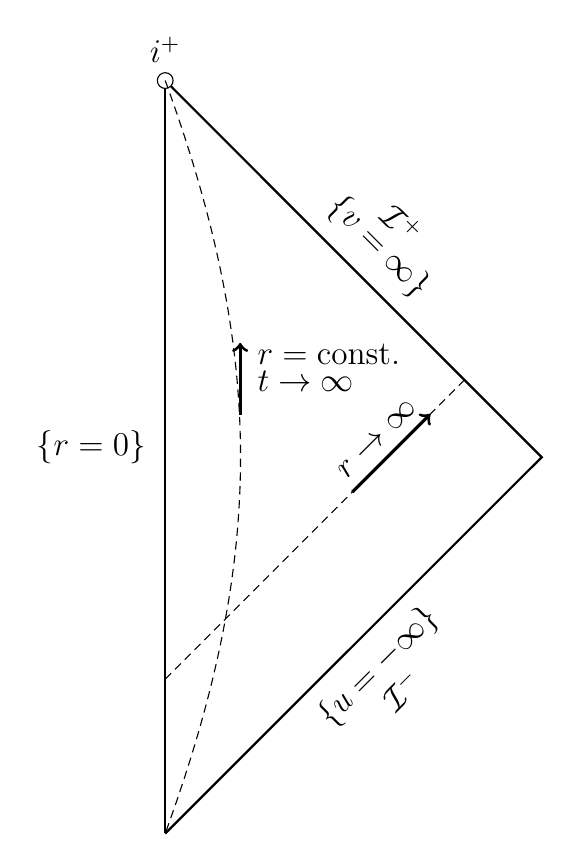
\begin{tikzpicture}[scale=1.4]
\coordinate (n1) at (0,0) {};
\node[circle, label= above:{\large$i^+$}, draw, inner sep =0, minimum size = .2cm] (n2) at (90:2.83) {};

\draw[thick] (n1) -- (n2);
\draw[thick] (n2) --(45:2);


\draw[thick] (45:2) -- +(-45: 2.83) -- (-90:4);
\node[label = {[rotate=45]below:\large$\{u=-\infty\}$}] at ($(-90:4) + (45:2.5)$) {};
\node[label = {[rotate=45, yshift=-.5mm]below:\large$\mathcal{I}^-$}] at ($(-90:4) + (45:2.5)+(-45:.3)$) {};
\node[label = left:{\large$\{r=0\}$}] at (-90:.5) {};

\draw[thick] (n1) -- +(-90:4); 

\node[label = {[rotate = -45]above:\large$\{v=\infty\}$}] at ($(90:2.83) + (-45:2.5)$) {};
\node[label = {[rotate = -45, yshift=.5mm]above:\large$\mathcal{I}^+$}] at ($(90:2.83) + (-45:2.5) + (45:.3)$) {};

\draw[densely dashed] (-90:2.6) -- ($(-90:2.6) + (45:3.85)$);
\draw[thick, ->,line width=.4mm]  ($(-90:2.6) + (45:2.4)$)--($(-90:2.6) + (45:3.4)$);
\node[label = {[rotate = 45, yshift=-.5mm, xshift = -.2mm]above:\large$r\rightarrow \infty$}] at ($(-90:2.6) + (45:2.85)$) {};

\draw[densely dashed] (90:2.83) to[out=-70, in = 70] (-90:4);
\draw[thick,->, line width=.4mm] (.68,-.2) -- ($(.68,0) + (90:.45) $);
\node[label={right:{  \large$r=\text{const.}$ }}] at (.66,.35) {};
\node[label={right:{  \large$t \rightarrow \infty$ }}] at (.66,.1) {};



\end{tikzpicture}

\end{document}